\documentclass[tikz,border=5mm]{standalone}
\usepackage{amsmath,amssymb}
\usetikzlibrary{shapes.arrows}

\begin{document}

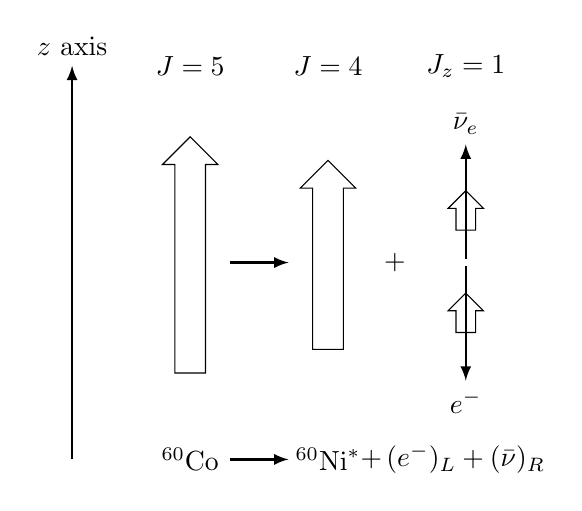
\begin{tikzpicture}[>=latex]

% Eje z
\draw[->, thick] (0,0) -- (0,5) node[above] {$z$ axis};

% Flechas para J=5
\node[single arrow, draw=black, fill=white, 
      minimum width = 20pt, 
      minimum height=30mm, 
      single arrow head extend=0.1cm, % Ajusta la longitud de la cabeza de la flecha
      rotate=90] at (1.5, 2.5) {}; % Rota la flecha 90 grados para que apunte hacia arriba
\node at (1.5, 5) {$J=5$};

% Flechas para J=4

\node[single arrow, draw=black, fill=white, 
      minimum width = 20pt, 
      minimum height=24mm, 
      single arrow head extend=0.1cm, % Ajusta la longitud de la cabeza de la flecha
      rotate=90] at (3.25, 2.5) {}; % Rota la flecha 90 grados para que apunte hacia arriba
\node at (3.25, 5) {$J=4$};

% Transición
\draw[->, thick] (2,2.5) -- (2.75,2.5);

% Flechas electrón y neutrino

\node[single arrow, draw=black, fill=white, 
      minimum width = 10pt, 
      minimum height=5mm, 
      single arrow head extend=0.1cm, % Ajusta la longitud de la cabeza de la flecha
      rotate=90] at (5, 3.1) {}; % Rota la flecha 90 grados para que apunte hacia arriba

\node[single arrow, draw=black, fill=white, 
      minimum width = 10pt, 
      minimum height=5mm, 
      single arrow head extend=0.1cm, % Ajusta la longitud de la cabeza de la flecha
      rotate=90] at (5, 1.8) {}; % Rota la flecha 90 grados para que apunte hacia arriba

\draw[thick, ->] (5,2.55) -- (5,4) node[above] {$\bar{\nu}_e$};
\draw[thick, ->] (5,2.45) -- (5,1) node[below] {$e^-$};

\node at (1.5, 0) {$^{60}\text{Co}$};
\node at (3.25, 0) {$^{60}\text{Ni}^*$};
\node at (5, 0) {$(e^{-})_L+(\bar{\nu})_R$};
\node at (4.1, 2.5) {+};
\node at (3.8, 0) {+};
\draw[->, thick] (2,0) -- (2.75,0);

% Etiqueta para J_z = 1
\node at (5,5) {$J_z = 1$};

\end{tikzpicture}

\end{document}
